\section{Configuración de agente en Linux}
Una vez que se realizó la instalación de Observium, continuamos con la instalación de la máquina virtual en Linux, en este caso, se utilizó Linux de forma nativa por lo cual pasamos directamente a la instalación de los paquetes ``SNMP'' y ``SNMPD'' por medio de la instrucción en consola:
\begin{itemize}
\item \textbf{sudo apt-get install snmp snmpd}
\end{itemize}
Posteriormente, se realizó la configuración del protocolo SNMP por medio del comando:
\begin{itemize}
\item \textbf{snmpconf $-$ r none $-$ g basic \_ setup}
\end{itemize}
Se puede observar en la figura \ref{image:snmp1} el procedimiento que nos apareció al ejecutar el comando anterior. A continuación se enlistarán las opciones que fueron seleccionadas en el transcurso de dicha configuración:
\begin{itemize}
\item Configurar la información devuelta en el sistema del grupo de la MIB.
\item Ingresamos un nombre para el almacenamiento del sistema.
\item Agregamos un correo electrónico.
\item Seleccionamos que no deseabamos configurar el valor de sysService.
\item Sí configuramos el agente de control de acceso.
\item No permitimos el acceso basado en usuario SNMPv3 de solo escritura.
\item No permitimos el acceso basado en usuario SNMPv3 de solo lectura.
\item Sí permitimos el acceso de la comunidad SNMPv1/v2c de lectura$-$escritura.
\item Añadimos un nombre a la comunidad de acceso de lectura$-$escritura.
\item Seleccionamos que no deseabamos agregar otra línea a rwcommunity.
\item Por último, no permitimos que la comunidad SNMPv1/v2c tuviera acceso de solo lectura.
\end{itemize}
\FloatBarrier
\begin{figure}[htbp!]
		\centering
			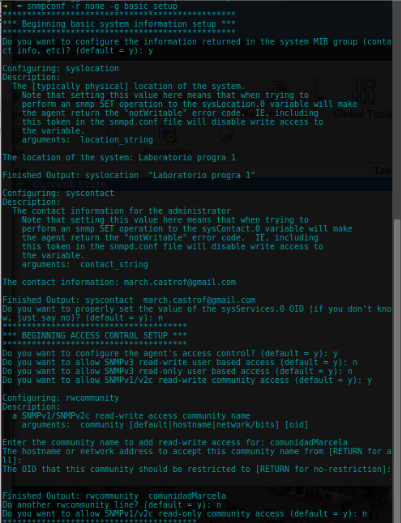
\includegraphics[width=.9 \textwidth]{images/snmpconf1}
		\caption{Configuración de snmp (1).}
		\label{image:snmp1}
\end{figure}
\FloatBarrier

Una vez finalizada toda la configuración básica, continuamos con la siguiente parte de la configuración mostrada en la figura \ref{image:snmp2}, en la cual se indicaron únicamente dos partes:
\begin{itemize}
\item No se configuró si el agente enviaría traps (trampas).
\item No se configuró la habilidad al agente para monitorear el sistema.
\end{itemize}
Es importante recalcar que una vez finalizadas estas dos acciones, se muestra que el archivo nombrado como \textbf{snmpd.conf} fue creado pues fue el utilizado posteriormente.
\FloatBarrier
\begin{figure}[htbp!]
		\centering
			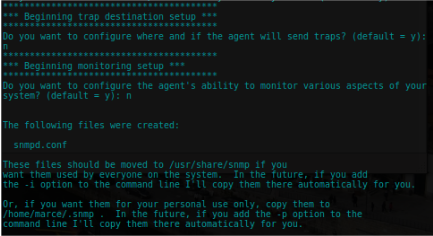
\includegraphics[width=.9 \textwidth]{images/snmpconf2}
		\caption{Configuración de snmp (2).}
		\label{image:snmp2}
\end{figure}
\FloatBarrier

Como se mencionó anteriormente, ya que se generó nuestro archivo de la configuración, se cambió el lugar de almacenamiento a la carpeta correcta por medio del comando:
\begin{itemize}
\item \textbf{sudo mv snmpd.conf $/$etc$/$snmp$/$snmpd.conf}
\end{itemize}
Y una vez que este fue almacenado debidamente, se reinició el servicio snmpd mediante la instrucción:
\begin{itemize}
\item \textbf{sudo service snmpd restart}
\end{itemize}
Y finalmente, por medio del comando:
\begin{itemize}
\item \textbf{nano /etc/snmp/snmpd.conf}
\end{itemize}
pudimos acceder al archivo mostrado en la figura \ref{image:snmp} en el cual podemos observar todo lo que se fue configurando y el cual es de mucha utilidad en caso de que hayamos olvidado el nombre de nuestra comunidad por ejemplo.
\FloatBarrier
\begin{figure}[htbp!]
		\centering
			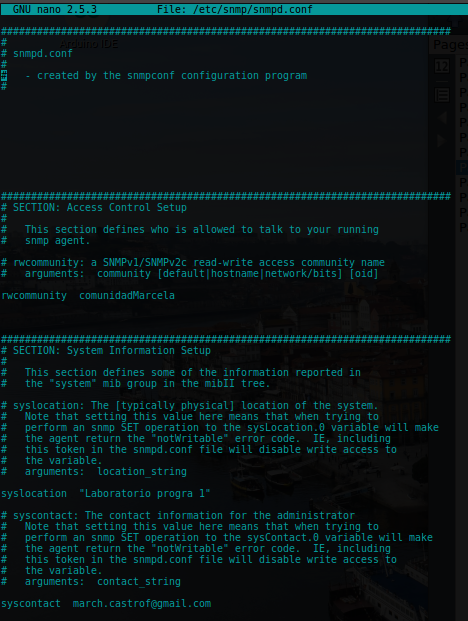
\includegraphics[width=.9 \textwidth]{images/snmpconf}
		\caption{Archivo de configuración finalizado.}
		\label{image:snmp}
\end{figure}
\FloatBarrier

Después regresamos a nuestro gestor de Observium en el cual abrimos nuestro archivo de hosts haciendo uso de la instrucción:
\begin{itemize}
\item \textbf{nano /etc/hosts}
\end{itemize}
mismo que nos abrirá el archivo mostrado en la figura \ref{image:hosts} en el cual agregamos la ip de nuestro sistema operativo Linux y un nombre identificador.
\FloatBarrier
\begin{figure}[htbp!]
		\centering
			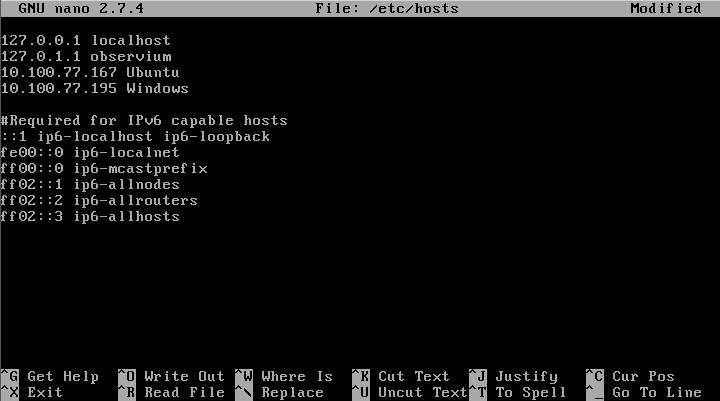
\includegraphics[width=.9 \textwidth]{images/hosts}
		\caption{Archivo de hosts Observium.}
		\label{image:hosts}
\end{figure}
\FloatBarrier
Guardamos y salimos para finalmente probar el funcionamiento de nuestra conexión mediante un ping más el nombre identificador escrito que en este caso fue Ubuntu para obtener una la respuesta mostrada en la figura \ref{image:ping}
\FloatBarrier
\begin{figure}[htbp!]
		\centering
			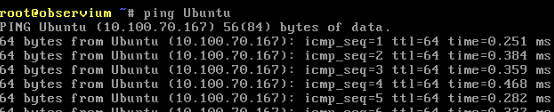
\includegraphics[width=.9 \textwidth]{images/ping}
		\caption{Ping a Linux.}
		\label{image:ping}
\end{figure}
\FloatBarrier

Por último, entramos a nuestra dirección de Observium en el navegador para añadir un dispositivo para monitorearlo como se observa en la figura \ref{image:device}, esto añadiendo un hostname que en este caso fue \textbf{Ubuntu} y una comunidad SNMP, misma que debe ser el nombre de la comunidad que elegimos poner en nuestro archivo de configuración que fue\textbf{comunidadMarcela}.
\FloatBarrier
\begin{figure}[htbp!]
		\centering
			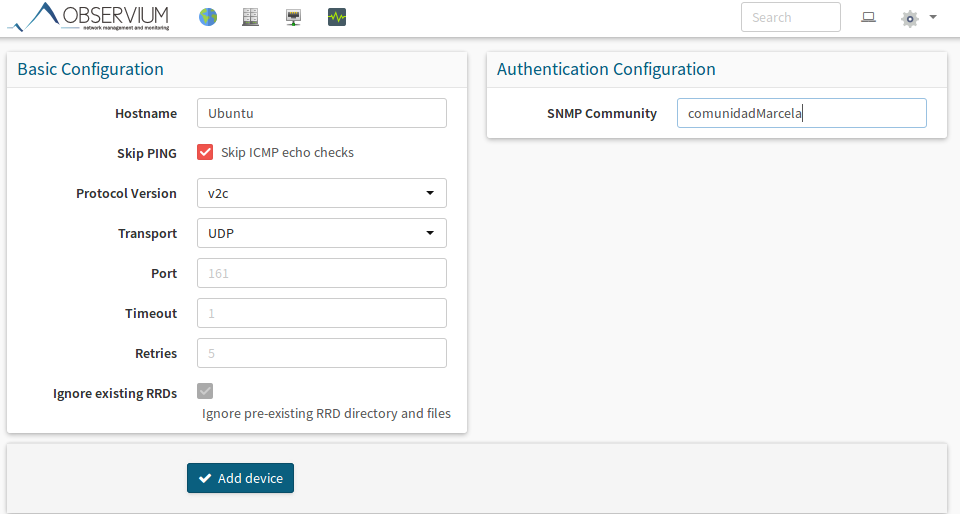
\includegraphics[width=.9 \textwidth]{images/device}
		\caption{Agente añadido.}
		\label{image:device}
\end{figure}
\FloatBarrier

Posteriormente, volvimos a la pestaña de Devices, seleccionamos All devices y aquí encontramos nuestro agente de Ubuntu como vemos en la figura \ref{image:deviceinfo}, mismo que al seleccionar nos muestra las diferentes gráficas e información de este.
\FloatBarrier
\begin{figure}[htbp!]
		\centering
			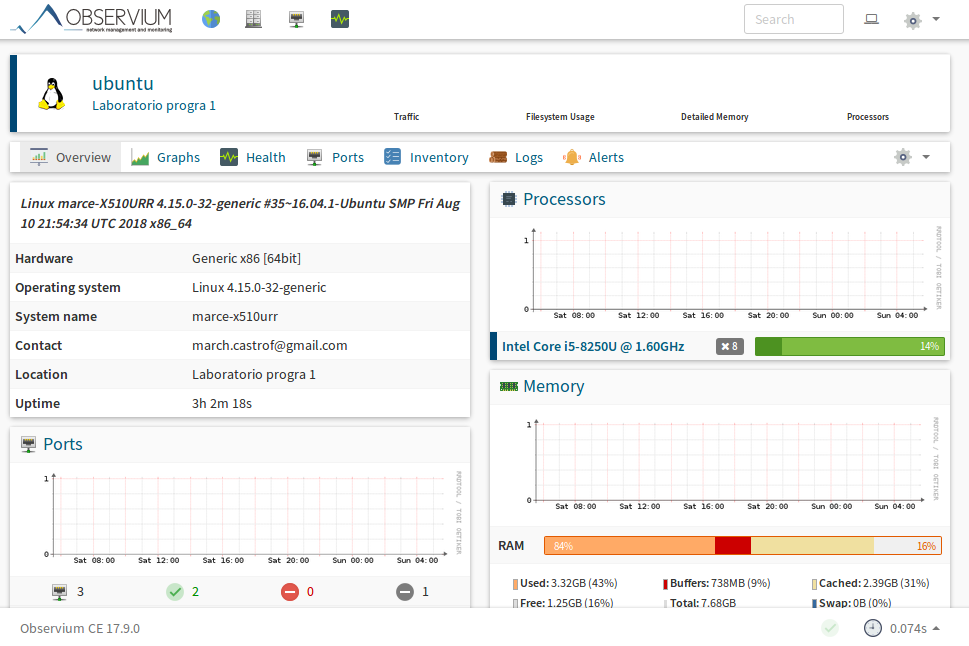
\includegraphics[width=.9 \textwidth]{images/deviceinfo}
		\caption{Información del agente.}
		\label{image:deviceinfo}
\end{figure}
\FloatBarrier